\section{Einführung}

\subsection{Grundbegriffe}

\begin{defi}{Datenkommunikation}

    Die \emph{Datenkommunikation} beschäftigt sich mit dem immateriellen Transport digitaler Daten zwischen Endsystemen.

    Hierbei sind alle benötigten Verfahren und Regeln Bestandteil der Datenkommunikation.

    Vorteile durch Datenkommunikation sind:
    \begin{itemize}
        \item zurückgreifen auf fremde bzw. entfernte Ressourcen und Daten
        \item Kostensenkung durch gemeinsame Nutzung von Betriebsmitteln
        \item Informationsgewinn durch entfernten Zugriff
    \end{itemize}

    Dazu benötigt es:
    \begin{itemize}
        \item Effiziente Methoden zum Datenaustausch zwischen Kommunikationspartnern
        \item Absprachen bzw. Regeln zur gemeinsamen Nutzung der Infrastruktur
        \item Kommunikationsdienste zur Übertragung von Informationen in verteilten Umgebungen
    \end{itemize}
\end{defi}

\begin{defi}{Kommunikationssystem}
    Im engeren Sinn ist ein \emph{Kommunikationssystem} eine Einrichtung bzw. eine Infrastruktur für die Übermittlung von Informationen.

    Kommunikationssysteme stellen dazu Nachrichtenverbindungen zwischen mehreren Endstellen her.
\end{defi}

\subsection{Kommunikationsmodelle}

\begin{defi}{Klassische Client-Server-Architektur}
    \emph{Server} sind langlebige Prozesse, welche auf Anfragen von Clients warten und diese abarbeiten.

    \emph{Clients} stellen zu beliebigen Zeiten Anfragen und warten auf die Antwort.
    Die Rolle ist damit zumeist beendet.

    \begin{center}
        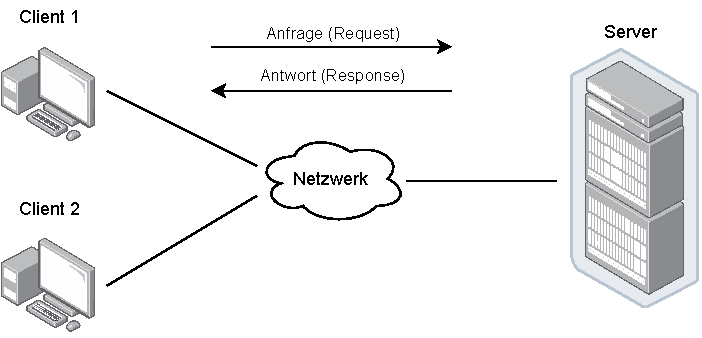
\includegraphics[width=0.75\textwidth]{includes/figures/defi_client_server.pdf}
    \end{center}
\end{defi}

\begin{bonus}{Dienst}
    Ein \emph{Dienst} wird von einem Verbund von Servern erbracht, durch den sich erst die Gesamtsicht ergibt.
    Ggf. merkt der Client nichts von dem Verbund.

    \begin{center}
        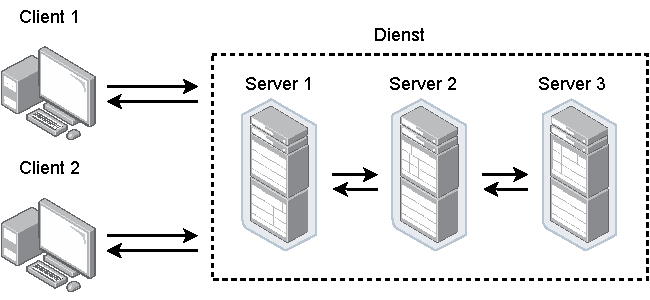
\includegraphics[width=0.6\textwidth]{includes/figures/bonus_dienst.pdf}
    \end{center}
\end{bonus}

\begin{bonus}{Proxy}
    Ein \emph{Proxy} dient zum Zwischenspeichern oder Anonymisieren von Anfragen auf der Clientseite, oder zum Lastbalanzieren auf der Serverseite.

    \begin{minipage}[t]{.5\textwidth}
        Forward Proxy:
    \end{minipage}%
    \begin{minipage}[t]{.5\textwidth}
        Reverse Proxy:
    \end{minipage}

    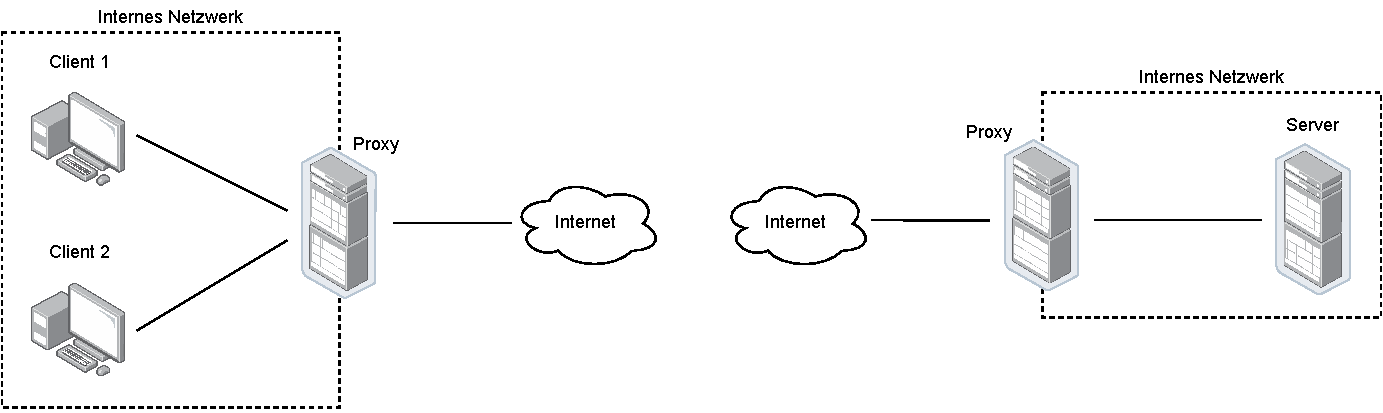
\includegraphics[width=\textwidth]{includes/figures/bonus_proxy.pdf}
\end{bonus}

\begin{defi}{Peer-to-Peer}
    In einem reinen \emph{Peer-to-Peer-Netz} sind alle Computer gleichberechtigt und können sowohl Dienste in Anspruch nehmen, als auch zur Verfügung stellen.

    Sobald die Peers, die die gesuchten Objekte halten, in dem P2P-System identifiziert wurden, wird die Datei (in Dateitauschbörsen) direkt, d. h. von Peer zu Peer, übertragen.
    Es existieren unterschiedliche Verteilungsstrategien, welche Teile der Datei von welchem Peer heruntergeladen werden soll, z. B. BitTorrent.

    \centering
    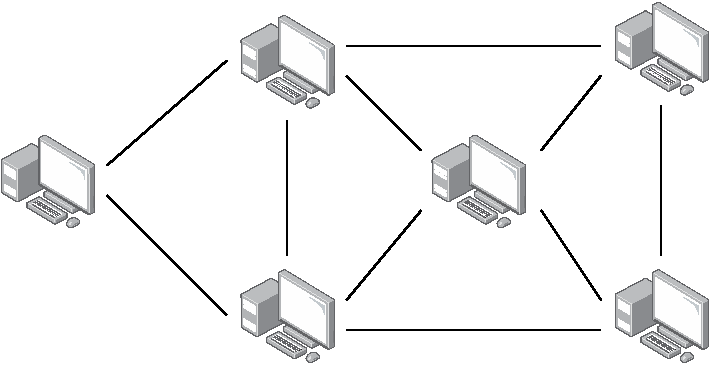
\includegraphics[width=.5\textwidth]{includes/figures/defi_peer_to_peer.pdf}
\end{defi}

\subsubsection{Klassifikation nach Übertragungstechnik}

\begin{defi}{Point-to-Point-Verbindung}
    Bei einer \emph{Point-to-Point-Verbindung} ist ein Paar von Rechnern durch eine direkte Leitung verbunden, ohne dass ein anderer Rechner diese Leitung nutzen kann.
    Man unterscheidet:

    \begin{tabularx}{\textwidth}{|l|X|X|}
        \hline
        Bezeichnung         & Beschreibung                                                                                & Beispiele                        \\
        \hline
        \hline
        \emph{Simplex}      & Daten können in nur eine Richtung übertragen werden, diese Technik ermöglicht keine Antwort & Rundfunk, Pager                  \\
        \hline
        \emph{Halbduplex}   & Daten können abwechselnd, aber nicht gleichzeitig, in beide Richtungen fließen              & Wechselsprechanlage, USB bis 2.0 \\
        \hline
        \emph{Vollduplex}   & Daten können in beide Richtungen gleichzeitig übertragen werden.                            & Gegensprechanlage, USB ab 3.0    \\
        \hline
        \emph{Dual-Simplex} & ähnlich Vollduplex, aber getrennte Sende- und Empfangswege                                  & PCI Express, Serial ATA          \\
        \hline
    \end{tabularx}
\end{defi}

\begin{defi}{Multi-Access-Netz}
    Bei einem \emph{Multi-Access-Netz} teilen sich mehrere Rechner einen Übertragungskanal.

    Damit Daten trotzdem an den richtigen Empfänger gesendet werden, müssen sie mit einer Zieladresse versehen werden.

    Daten werden in Übertragungseinheiten (Frames) eingeteilt und mit der Empfängeradresse ausgewiesen.\footnote{Sollen alle Stationen gleichzeitig eine Nachricht erhalten, so werden Broadcast-Adressen verwendet.}
\end{defi}

\subsubsection{Klassifikation nach Verbindungsart}

\begin{defi}{Statisches Netz}
    In einem \emph{statischen Netz} befinden sich fest verdrahtete Point-to-Point-Verbindungen oder Multi-Access-Netze.

    Dabei besitzt jeder Knoten eine feste Anzahl von Nachbarn oder einen Zugang zu einem Multi-Access-Netz.
\end{defi}

\begin{defi}{Dynamisches Netz}
    In einem \emph{dynamischen Netz} enthalten die Verbindungen konfigurierbare Schaltelemente.

    Diese können dynamisch vermitteln durch Leitungsvermittlung\footnote{Man sagt \enquote{ein Weg wird geschaltet}.}.

    Dabei ist ein ein- oder mehrstufiger Aufbau möglich.
\end{defi}

\subsubsection{Klassifikation nach Topologieeigenschaften}

\begin{defi}{Durchmesser}
    Der \emph{Durchmesser} eines Netzes gibt an, wie groß der maximale Abstand zweier Knoten, d. h. die Anzahl von Kanten (Links), die auf einem kürzesten Pfad (Route) zwischen Knoten genutzt werden muss.

    Das Ziel ist ein möglichst kleiner Durchmesser und damit ein möglichst kleiner Zeitbedarf für Übertragungen.
\end{defi}

\begin{defi}{Bisektionsweite}
    Die \emph{Bisektionsweite} eines Netzes gibt die minimale Anzahl von Kanten an, die man entfernen muss, um ein Netz mit $N$ Knoten in zwei isolierte Teile mit jeweils $\frac{N}{2}$ Knoten zu teilen.

    Das Ziel ist eine möglichst große Bisektionsweite zur Verbesserung der Fehlertoleranz.
\end{defi}

\begin{defi}{Grad}
    Der \emph{Grad} eines Netzes entspricht dem größten Grad eines Knotens.

    Der Grad eines Knotens wiederum ist die Anzahl ausgehender Kanten, d. h. die Anzahl der Nachbarn des Knotens.\footnote{Haben alle Knoten den gleichen Knotengrad, so spricht man von einem \emph{regulären Netz}.}

    Das Ziel ist ein möglichst kleiner Grad des Netzes, da die Kosten mit dem Grad steigen.
\end{defi}

\begin{defi}{Netzwerktopologie}
    \centering
    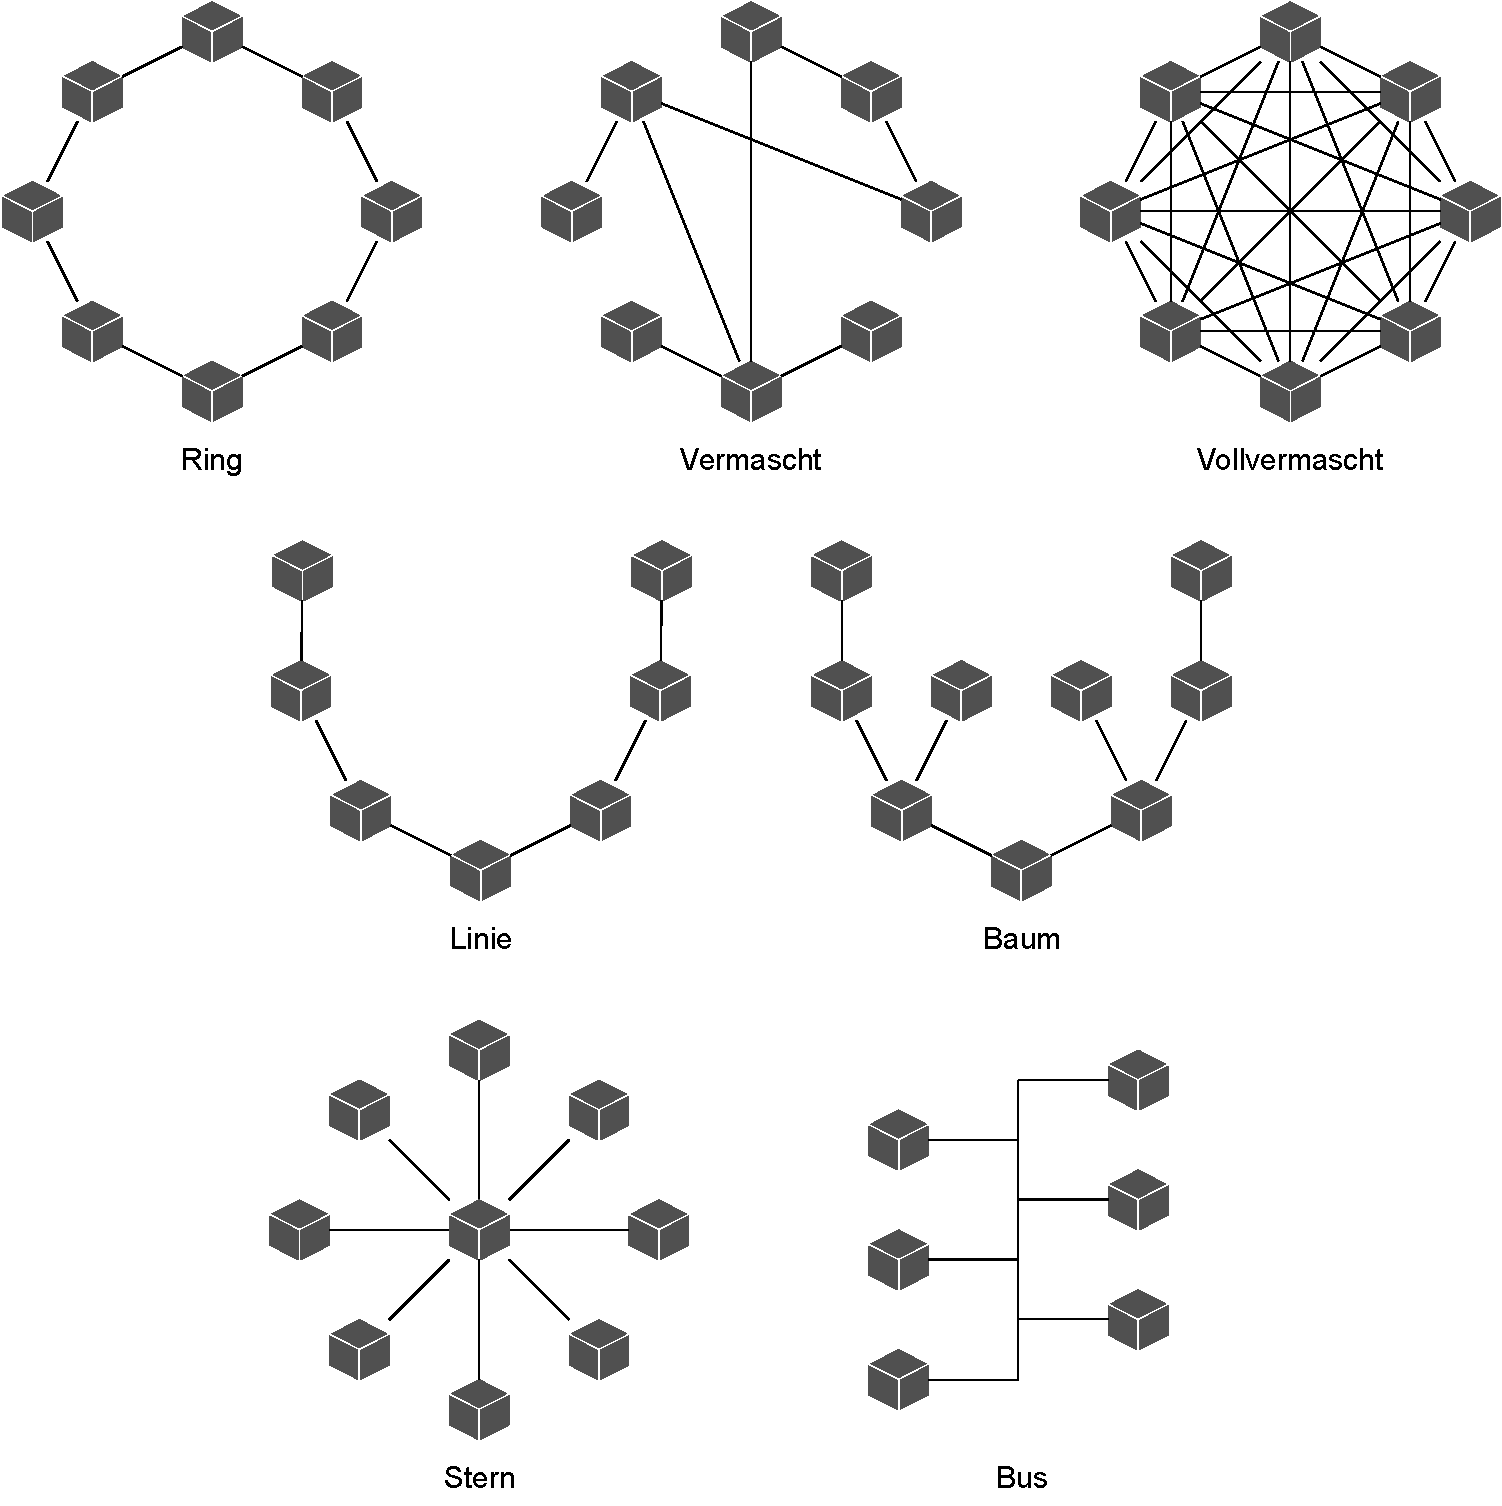
\includegraphics[width=\textwidth]{includes/figures/defi_topologien.pdf}

    \begin{tabularx}{\textwidth}{|X|l|l|l|l|}
        \hline
        Topologie                                                                                                                                      & Durchmesser       & Bisektionsweite     & Grad           & Regulär \\
        \hline \hline
        \emph{Ring}                                                                                                                                    & $\nicefrac{N}{2}$ & $2$                 & $2$            & Ja      \\
        \hline
        \emph{Vollvermascht}\footnote{\emph{Vermascht} ist analog. Da dort aber keine festen Regeln sind, sind die Kennzahlen schwierig zu bestimmen.} & $1$               & $\nicefrac{N^2}{4}$ & $N-1$          & Ja      \\
        \hline
        \emph{Linie}                                                                                                                                   & $N-1$             & $1$                 & $1$ bzw. $2$   & Nein    \\
        \hline
        \emph{Baum} (binär)                                                                                                                            & $2 \log_2 N$      & $1$                 & $1$ oder $2$   & Nein    \\
        \hline
        \emph{Stern}                                                                                                                                   & $2$               & $(1)$               & $1$ bzw. $N-1$ & Nein    \\
        \hline
        \emph{Bus}                                                                                                                                     & $1$               & $(1)$               & $(1)$          & (Ja)    \\
        \hline
    \end{tabularx}

    Für Details, siehe \ref{ssec:netztopologien}.
\end{defi}

\subsubsection{Klassifikation nach Ausdehnung}

\begin{defi}{Local Area Network (LAN)}
    Ein \emph{Local Area Network (LAN)} ist eine Kommunikationsinfrastruktur für einen begrenzten geographischen Bereich (10 Meter bis wenige Kilometer).

    Typischerweise erfolgt die Verkabelung eines LANs ab einer gewissen Größe als strukturierte Verkabelung.
    Ethernet ist der am weitesten verbreitete Standard.
\end{defi}

\begin{defi}{Metropolitan Area Network (MAN)}
    Ein \emph{Metropolitan Area Network (MAN)} überbrückt größere Distanzen als ein LAN, z. B. den Bereich einer Stadt.

    Üblicherweise verbindet ein MAN zahlreiche LANs und verwendet dazu eine Backbone-Technologie, die meist in Glasfasertechnik realisiert ist.
    Ein MAN kann eine Ausdehnung von bis zu 100 km haben.

    MANs werden oft von international tätigen Telekommunikationsfirmen aufgebaut, die per MAN verkabelte Metropolen wiederum in einem Wide Area Network (WAN) national oder in einem Global Area Network (GAN) international vernetzen.
\end{defi}

\begin{defi}{Wide Area Network (WAN)}
    Ein \emph{Wide Area Network (WAN)} ist ein Rechnernetz, das sich im Unterschied zu einem LAN oder MAN über einen sehr großen geografischen Bereich erstreckt.

    Die Anzahl der angeschlossenen Rechner entsprechen dem Maximum von IPv4 oder IPv6.
    WANs erstrecken sich über Länder oder sogar Kontinente.

    WANs werden benutzt, um verschiedene LANs, aber auch einzelne Rechner miteinander zu vernetzen.

    Einige WANs gehören bestimmten Organisationen und werden ausschließlich von diesen genutzt.
    Andere WANs werden durch Internetdienstanbieter errichtet oder erweitert, um einen Zugang zum Internet anbieten zu können.
\end{defi}

\begin{defi}{Global Area Network (GAN)}
    Unter einem \emph{Global Area Network (GAN)} versteht man ein Netz, das über unbegrenzte geographische Entfernungen mehrere Wide Area Networks verbinden kann.
    Dies kann zum Beispiel die Vernetzung weltweiter Standorte eines internationalen Unternehmens sein.

    Oft wird bei einem GAN Satelliten- oder Glasfaserübertragung eingesetzt.

    GAN ist nicht die direkte Bezeichnung für das Internet, da es theoretisch mehrere GANs abgeschottet und unabhängig geben kann, das Internet jedoch eine globale Vernetzung ohne (maßgebliche) Unterteilungen ist.
    So ist das Internet ein GAN, aber nicht jedes GAN wird Internet genannt.
\end{defi}

\subsubsection{Klassifikation nach Netzkomponenten}

\begin{defi}{Switch}
    Ein \emph{Switch} hat mehrere Anschlüsse, über die Rechner miteinander verbunden werden können.

    Er merkt sich, welcher Rechner an welchem Anschluss angeschlossen ist (Adresse der Netzwerkkarte) und kann Daten gezielt an einen Anschluss weiterleiten.

    Der Switch kennt nur Rechner, die direkt an ihn angeschlossen sind.
\end{defi}

\begin{defi}{Router}
    Will man Daten an weit entfernte Kommunikationspartner schicken, gibt es meist mehrere mögliche Wege, die man nehmen kann.

    \emph{Router} verwalten globale Adressinformationen, kennen kürzeste Wege zu allen Rechnern und können Daten gezielt in andere Netze weiterleiten.
\end{defi}

\begin{defi}{Backbone}
    Als \emph{Backbone} bezeichnet man eine Menge von Rechnern, die miteinander verbunden sind, um kleinere Netze miteinander zu koppeln und so den Datenaustausch zu ermöglichen.
\end{defi}